%==================================================================================================
%   LUKES THESIS TEMPLATE 1.2
%   -------------------------
%   This template is based upon the offcial IMM PhD Thesis template, it is enhanced with a number
%   of new features and a number of errors have fixed. This template is intended to be complied to
%   PDF using PDFLATEX and is tested using the MiKTeX 2.9 LaTeX distribution.
%   It is based on the official DTU-IMM Thesis template by Finn Kuno Christensen in 2009.
%   Small bugfixes by Kasper Laursen in 2012 and 2013.
%   Small updates by Finn Kuno Christensen/Henning Christiansen in 2015.
%   -------------------------
%   Last Updated: 2015-01-08
%==================================================================================================
%
%==================================================================================================
% DOCUMENT SETUP
%==================================================================================================
\documentclass[10pt,twoside]{book}                  %Official DTU-IMM Thesis document setup
%
%Set to 'print' for printed version, use 'net' for online version
\def\thesisversion{print}
%
%==================================================================================================
% PACKAGES
%==================================================================================================
\usepackage{LukeThesis}                             %Import Thesis base style
%input{PhDMacros}                                   %Thesis specific macros
%
%==================================================================================================
% THESIS PROPERTIES (Modifiy these fields with your details)
%==================================================================================================
\def\thesisauthor{Jonas Bruun Hubrechts}                     %Author
\def\thesistitle{Something something}               %Title
\def\thesishandin{01-July}                       %Submission date (Day-Month}
\def\thesisdegree{M.Sc.}                            %Degree ('B.Eng', 'B.Sc.', 'M.Sc.' or 'PhD')
\def\thesisyear{2024}                               %Submission year
\def\thesisnumber{????}                             %DTU-IMM Serial number (do not include year)
\def\thesisISSN{0000-0000}                          %ISSN number
\def\thesiskeywords{Keywords are, comma separated}  %PDF keywords
\derivethesisprops                                  %Derive dependent properties
%
%==================================================================================================
% SECTION NUMBERING SETUP
%==================================================================================================
\setcounter{tocdepth}{2}                            %2 adds sections up to subsections
\setcounter{secnumdepth}{3}                         %Subsubsections get a number when this is 3
%
%==================================================================================================
% THESIS STRUCTURE  (Modifiy to include more chapters etc)
%==================================================================================================
\begin{document}
%------------------------
%Pre-frontmatter material
%------------------------
\prefrontmatter
%--------------------
%Frontmatter material
%--------------------
\frontmatter
\pagenumbering{roman}                               %Set frontmatter numbering style
\chapter{Abstract}


% Introduction
% Purpose
% Method
% Results
% Conclusion + future works
Casual relations between processes are a core issue for effective control of production systems. In particular, it is paramount to understand how variations, such as delays, propagate through the production system for feasible and robust scheduling of processes.

This thesis aims to uncover such causal relations from observations of production flow runs. To obtain the above, we shall present a method for network deconvolution, where direct and indirect effects are separated. The algorithm's robustness is explored in depth, focusing primarily on the influence of noise. Moreover, we shall extend the algorithm to work with mixed random variables, which is crucial for delay modeling, and discuss in detail how to estimate mutual information for such joint distributions. Furthermore, topological assumptions are considered and shown to improve the method's accuracy.

Applying the method to controlled examples with known causal structures, we observe that chainlike causal structures can be tough to recover. However, assuming a topological order, this problem is greatly alleviated. More complex causal structures are considered, where the method also performs well. In particular, with only a few hundred observations, the algorithm can recover the causal structure.

Finally, the method is applied to a dataset from a simulated pharmaceutical production system. We show how the framework functions in practice and demonstrate the robustness of the inferred causal structure by including more or fewer variables. In particular, we shall observe that almost all delays are unexplained by previous incidents.

Based on the results of this thesis, the algorithm combined with mutual information as a measure of similarity appears to constitute a promising and generally applicable framework for causal discovery. However, observations regarding possible optimizations of estimating mutual information from data are noted. Namely, for random variables that are almost perfectly descriptive of each other, the information is shown to be underestimated. This error results in a bias but is, in most situations, not a problem.



% \newpage


% \cite{An_effective_approach_for_causal_variables_analysis_in_diesel_engine_production_by_using_mutual_information_and_network_deconvolution}
% The effective control of the power consistency, which is one of the most important quality indicators of diesel engine, plays a decisive role for improving the competitiveness of the products. The widely used sensors and other data acquisition equipment make the “data-driven quality control” become possible. 

% However, how to determine the highly related parameters with the engine power from massive captured manufacturing data and effectively discriminated the direct and indirect dependencies between these variables are still challenging. This paper proposed a feature selection algorithm named NMI-ND which uses network deconvolution (ND) to infer causal correlations among various diesel engine manufacturing parameters from the observed correlations based on normalized mutual information (NMI). The proposed algorithm is thoroughly evaluated through the experimental study by comparing it with other representative feature selection algorithms. The comparison demonstrates that NMI-ND performs better in both effectiveness and efficiency.



% \cite{Network-deconvolution-as-a-general-method-to-distinguish-direct-dependencies-in-networks}
% Recognizing direct relationships between variables connected
% in a network is a pervasive problem in biological, social and
% information sciences as correlation-based networks contain
% numerous indirect relationships.

% Here we present a general
% method for inferring direct effects from an observed
% correlation matrix containing both direct and indirect
% effects. We formulate the problem as the inverse of network
% convolution, and introduce an algorithm that removes the
% combined effect of all indirect paths of arbitrary length in
% a closed-form solution by exploiting eigen-decomposition
% and infinite-series sums. We demonstrate the effectiveness
% of our approach in several network applications: distinguishing
% direct targets in gene expression regulatory networks; recognizing
% directly interacting amino-acid residues for protein structure
% prediction from sequence alignments; and distinguishing
% strong collaborations in co-authorship social networks using
% connectivity information alone. In addition to its theoretical
% impact as a foundational graph theoretic tool, our results suggest
% network deconvolution is widely applicable for computing direct
% dependencies in network science across diverse disciplines.


% \cite{Nonparametric-copula-entropy-and-network-deconvolution-method-for-causal-discovery-in-complex-manufacturing-systems}
% To clarify the causality among process parameters is a core issue of data-driven production performance analysis and product quality optimization. The difculty lies in accurately measuring and distinguishing direct and indirect associations of complex manufacturing systems.

% In this work, the nonparametric-copula-entropy and network deconvolution method is proposed for causal discovery in complex manufacturing systems. Firstly, based on copula theory and kernel density estimation method, the nonparametric-copula-entropy is introduced to improve the accuracy of association measurement between parameters, and its superiority is verifed by comparing with the results of diferent association measurement methods. Then, the global association matrix is constructed by the nonparametric-copula-entropy, and network deconvolution method is employed to extract the direct information from the global association matrix. The proposed method is tested by using an open gene expression dataset. Finally, as an experimental application, the causal analysis for a diesel engine production line is carried out by the proposed method. The results show that the proposed method can reveal causal relationship between process parameters and quality parameters in the diesel engine production line well, which provide theoretical guidance and implementation approach for the optimal control of complex manufacturing system.                                   %English summary of Thesis
\markboth{}{}                                       %Set headings (left)(right)
\chapter{Summary (Danish)}
\begin{otherlanguage}{danish}

Målet for denne afhandling er at ...

\end{otherlanguage}                                   %Danish summary of Thesis
\markboth{}{}                                       %Set headings (left)(right)
\chapter{Preface}

This thesis corresponds to 30 ECTS credits and was prepared at DTU Compute in fulfilment of the requirements for acquiring an M.Sc. in Engineering.

A special thanks to my supervisors Tobias Overgaard, Nicolai Siim Larsen and Bo Friis Nielsen for their help and guidance throughout this study.

% The thesis deals with ...

% The thesis consists of ...
%==================================================================================================
% SIGNATURE AREA
%==================================================================================================
\vspace{20mm}
\begin{center}
    \hspace{20mm} Lyngby, \thesishandin-\thesisyear
    \vspace{5mm}
    \newline
  %Update signature image file in line below
    % \includegraphics[scale=0.2]{figures/Signature.png}
\end{center}
\begin{flushright}
    \thesisauthor
\end{flushright}
% % % EOF % % %




                                     %Preface
\markboth{}{}                                       %Set headings (left)(right)
\chapter{Acknowledgements}

I would like to thank my....

                            %Acknowledgements
\markboth{}{}                                       %Set headings (left)(right)
%------------------
% Table of contents
%------------------
\newpage\mbox{}\newpage
\chaptermark{Contents}
\pdfbookmark{\contentsname}{toc}
\renewcommand{\sectionmark}[1]{\markright{#1}}
\sectionmark{Contents}
\addtolength{\parskip}{-\baselineskip}
\tableofcontents
\addtolength{\parskip}{\baselineskip}
\renewcommand{\sectionmark}[1]{\markright{\thesection\ #1}}
%-------------
% Main content
%-------------
\mainmatter
% \documentclass[../Thesis.tex]{subfiles}
\graphicspath{{\subfix{../figures/}}}
\begin{document}
\chapter{Introduction By Jonas}

\textit{The following text is a message to the student and should be removed during the writing process.}

Please note the following instructions regarding an MSc thesis outlined in the study handbook:

``During the first month, the student is to submit a project plan outlining the objective of the thesis and justification for same to his/her supervisor. In the project plan, the student is also to take into account the overarching learning objectives listed above. When submitting the thesis, the student is to enclose a separate document presenting the original project plan and a revision of same, where appropriate. In addition, the document is to include a brief auto-evaluation of the project process.''

To learn more about the rules for an MSc thesis, please consult the rules for your own MSc programme at \url{http://sdb.dtu.dk}.

\section{Project plan}
We note that the contents of the project plan is also something we would like to see in the introductory chapter of your thesis. In fact, you can reuse your final project plan (possibly extended) as the introduction. If you prefer to write an introduction from scratch, it is, of course, important that it is consistent with the final project plan.

\section{The ``separate document''}
It is also important to note that the separate document containing
\begin{itemize}
    \item original project plan
    \item possibly revised project plan.
    \item brief self-evaluation
\end{itemize}
mentioned above will be passed on to the external examiner and since it contains the learning goals and the objectives for your thesis, it will be taken into account when your thesis is assessed.

\cite{Hoare78}

\cite{CK01}

\end{document}
                                  %Chapter 1
\subfile{Chapters/Chapter1.tex}
% \documentclass[../Thesis.tex]{subfiles}
\graphicspath{{\subfix{../figures/}}}
\begin{document}

\chapter{
    Problemformulering / Introduktion
}

In many production facilities, planning is a big part of maximizing some index. Whether this is production throughput over some time period and thus often also the economic surplus or some other key index, it is of great importance to have an underlying model to describe the observed variation. In particular in operational research, the schedules may drift in suboptimal ways if the variation is not considered.


Furthermore, from a salesman point of view, expected production and time intervals can be of great use when planning and also building production facilities. Namely, one might find that increasing the volume or efficiency of some part of the facility would increase the production throughput and profitability. This is also known as bottleneck analysis and require some understanding of the underlying mechanics and a stochastic model of this could improve the strength of such results.


Therefore, the primary objective of this paper/thesis is to investigate and model the yield and time of a production flow with focus on the pharmaceutical and chemical production industry. More precisely, we will be building a statistical model for a single process, with the purpose of being able to describe the variation in the yield of the production cycle and production times. This will then be used to analyze potential bottlenecks.

Furthermore, it will be interesting to construct a network of such processes as is typically the case in industry. We shall see how much can be said about such a network and what obstacles one may encounter when trying to analyze such networks which is this thesis will initially be treated as networks of queues.



% With the possibility  










\chapter{Ideer til hvad der skal laves}

Overall model for throughput of system. I.e. model the system as e.g. a system of queues and how much is produced at each step and this propagate. The important aspect is breakdown (extra processing time) and possibility of having to trowing out some production along the way, either due to error or some other (unforeseen) causes.

Need to investigate different ways of modelling this (starting with a simple system with no queuing, i.e. a single batch; this is what is done above). Discuss the pros and cons and how much information they preserve (aggregation models etc. may need to model so'me part of the system by throwing away)


\begin{itemize}
    \item \href{https://en.wikipedia.org/wiki/Petri_net}{Petri Net}
    \item ODE Stochastic Chemical Reaction (first order)
    % \item \href{https://onlinelibrary.wiley.com/doi/epdf/10.1002/ceat.270150109}{A Multiple State Stochastic Model for Deep-bed Filtration}
    \item \href{https://www.nature.com/articles/s41597-020-0455-1}{Database of pharmacokinetic time-series data}
    \item \href{https://search.r-project.org/CRAN/refmans/AppliedPredictiveModeling/html/ChemicalManufacturingProcess.html}{Chemical Manufacturing Process Data}
\end{itemize}

\end{document}
                                %Chapter 2
\appendix

\documentclass[../Thesis.tex]{subfiles}
\graphicspath{{\subfix{../figures/}}}
\begin{document}
\chapter{Appendix}

\section{Suicide data}
\begin{table}[H]
    \centering
    \begin{tabular}{cccccc}
1 & 25 & 40 & 83 & 123 & 256 \\
1 & 27 & 49 & 84 & 126 & 257 \\
1 & 27 & 49 & 84 & 129 & 311 \\
5 & 30 & 54 & 84 & 134 & 314 \\
7 & 30 & 56 & 90 & 144 & 322 \\
8 & 31 & 56 & 91 & 147 & 369 \\
8 & 31 & 62 & 92 & 153 & 415 \\
13 & 32 & 63 & 93 & 163 & 573 \\
14 & 34 & 65 & 93 & 167 & 609 \\
14 & 35 & 65 & 103 & 175 & 640 \\
17 & 36 & 67 & 103 & 228 & 737 \\
18 & 37 & 75 & 111 & 231 \\
21 & 38 & 76 & 112 & 235 \\
21 & 39 & 79 & 119 & 242 \\
22 & 39 & 82 & 122 & 256
    \end{tabular}
    \caption{The length of treatment of control patients in suicide study. The data originates from the Mental Health Enquiry (MHE) of England of Wales and was published in 1967.}
    \label{tab:suicide data}
\end{table}

\newpage
\section{Confidence interval for absolute correlation in bivariate Gaussian}\label{sec:bivar gauss abs correlation CI}
From \cite{Confidence-in-Correlation}, given a bivariate Gaussian, the confidence distribution of $\rho$ given the empirical correlation $r$ based on $n$ observations is given by
$$f\left(\rho \mid r,\nu\right) = \frac{\nu (\nu-1) \Gamma(\nu-1)}{\sqrt{2\pi} \Gamma(\nu + \frac{1}{2})} \frac{\left(1-r^2\right)^{\frac{\nu-1}{2}} \left(1-\rho^2\right)^{\frac{\nu-2}{2}} }{\left(1-r\rho\right)^{\frac{2\nu-1}{2}}} F\left(\frac{3}{2}, -\frac{1}{2}, \nu+\frac{1}{2}, \frac{1+r\rho}{2}\right)$$
where $F\left(a,b,c,z\right)$ is the Gaussian hypergeometric function and $\nu = n-1$. That is, given a sample correlation $r$, what is the confidence in $\rho$ in terms of a distribution. In the following figure, a sample correlation $r=0.8$ and $r=0$ has been used with varying number of observations (degrees of freedom) in figures \autoref{subfig:gaussian correlation dist 0.8} and \autoref{subfig:gaussian correlation dist 0} respectively.
\begin{figure}[h]
    \centering
    \begin{subfigure}[t]{0.49\linewidth}
        \centering
        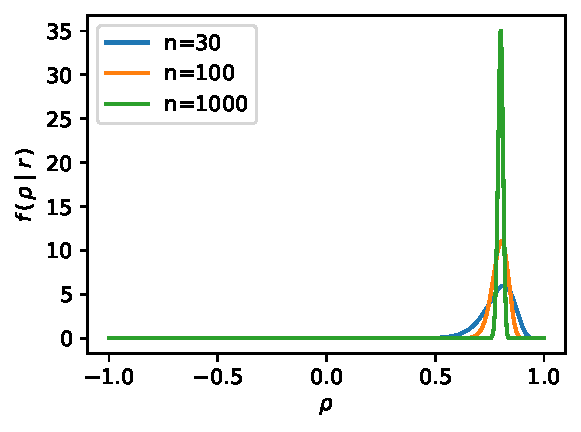
\includegraphics[width=\linewidth]{figures/Gaussian correlation confidence dist/density comparison r 0.8.pdf}
        \caption{}
        \label{subfig:gaussian correlation dist 0.8}
    \end{subfigure}%
    ~
    \begin{subfigure}[t]{0.49\linewidth}
        \centering
        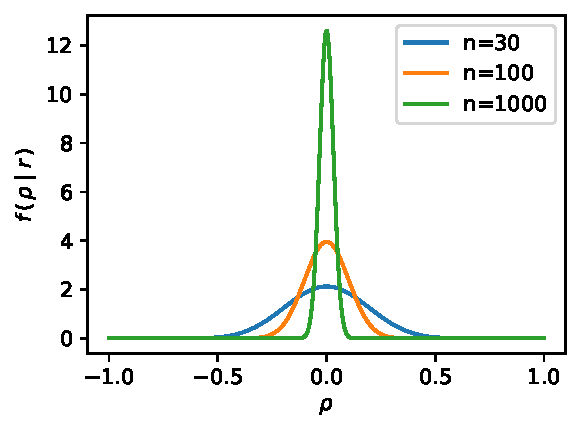
\includegraphics[width=\linewidth]{figures/Gaussian correlation confidence dist/density comparison r 0.pdf}
        \caption{}
        \label{subfig:gaussian correlation dist 0}
    \end{subfigure}
    \caption{$f\left(\rho \mid r, \nu\right)$ shown for $r=0.8$ and $r=0$ in (a) and (b) with $n\in \{30,100,1000\}$. As one would expect, the power i.e. the width of the peak decreases with increasing n and for correlations closer to $0$, the width is the largest.}
\end{figure}
A key property is that $f$ is \textit{even symmetric} in $\rho,\, r$. That is $f(\rho \mid r) = f(-\rho \mid -r)$. Thus, a confidence interval for $\rho$ given $r$ is the negative of the confidence interval given $-r$. In particular, if we only observe $|r|$, we can calculate a confidence interval for $\rho$ up to the sign of the bounds of the interval. Furthermore, as we want a CI for $|\rho|$, it does not matter if $r$ is negative or positive. Hence, without loss of generality, we assume that $r \geq 0$. At this point, to construct a confidence interval for $|\rho|$ we list the following desired properties. Firstly, it should be an exact confidence interval, meaning that for a given significance level $\alpha$, the CI includes the true value exactly $1-\alpha$ fraction of the times. Secondly, if for a given $r$, it can not be rejected that $\rho$ is 0, 0 should also be contained in the interval. Finally, if we reject that $\rho = 0$, we shall have $\alpha/2$ probability mass above and below the bounds of the interval. The above is enough to uniquely define a confidence interval in all cases. Before continuing with how this CI is calculated, we mention that as $r$ is an unbiased estimator of $\rho$, we would preferably want $|r| \in CI_{1-\alpha}\left(|\rho|\right)$ (where $CI_{1-\alpha}\left(|\rho|\right)$ denotes the $1-\alpha$ confidence interval for $|\rho|$). However, although this will in almost every scenario be the case, we can not be sure of this from the above properties and in fact examples with large $\alpha$ can be constructed such that $|r|$ lies just outside the constructed CI.

First, to conform with the second desired property, if it can not be rejected that $\rho = 0$ on a significance level $\alpha$, we will initially compute a CI for $\rho$ (not $|\rho|$) based on $r$ (wlog chosen to be non-negative). This CI will just be a symmetric CI in the sense that $\alpha/2$ of the probability mass will lie below the lower bound of the CI and above the upper bound of the CI respectively. If $0$ is contained in this CI, we can not reject that $\rho=0$ and vice versa on an $\alpha$ significance level. Thus, if $0$ is contained in this initial CI for $\rho$, we will start the CI for $|\rho|$ at $0$ and determine and upper bound $b$ such that $\alpha$ probability mass is above this $b$. Otherwise, we shall find $a$ and $b$ such that $\alpha/2$ probability mass is below $a$ and above $b$ respectively. Choosing $a$ and $b$ this way also conforms with the third property. Finally, to ensure that the CI contains exactly $1-\alpha$, we define $\tilde{f}$ as the reflected $f$ in $\rho$ such that
$$\tilde{f}\left(\rho_a \mid r_a, \nu\right) = f(\rho_a \mid r_a, \nu) + f(-\rho_a \mid r_a, \nu),\quad \rho_a,r \in [0,1]$$
where $\rho_a$ and $r_a$ is the absolute correlation and empirical correlation respectively. With this $\tilde{f}$, the density at $\rho_a$ is both the density for the negative and positive correlation ensuring that the $\tilde{f}$ has probability mass $1$. Thus, if $a=0$ (i.e. the CI must contain $0$), we find $b$ as the $1-\alpha$ percentile of $\tilde{f}$ and if $a\neq 0$, we take $a$ as the $\alpha/2$ percentile and $b$ as the $1-\alpha/2$ percentile of $\tilde{f}$.

As an example, suppose $r_a=0.06$ with $1000$ observations. Then a $95\%$ CI for $|\rho|$ is $[0, 0.11164]$ whereas if on had observed $r_a = 0.07$ the CI would be $[0.01071, 0.1314]$. These CI could then be used to test the absolute correlation of a bivariate Gaussian i.e. for $r_a = 0.07$ based on $1000$ observations would be rejected as stemming from a Gaussian with absolute correlation $0.01$ on a $5\%$ significance level.


\newpage
\section{Gaussian chain deconvolution}

\begin{figure}[H]
    \centering
    \begin{subfigure}[t]{0.49\textwidth}
        \centering
        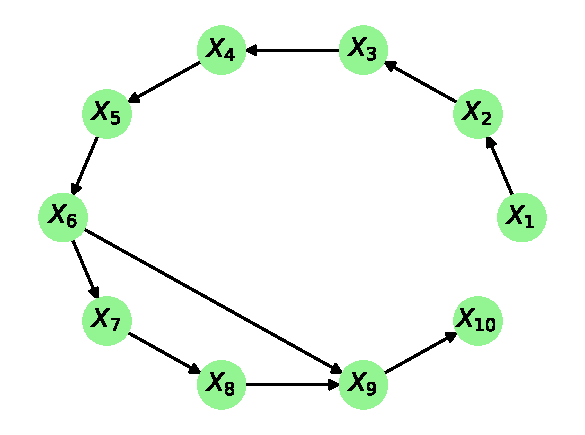
\includegraphics[width=.95\linewidth]{figures/Gaussian Chain Theoretical/Chain graph from triangular G obs - MI - cutoff 2e-2.pdf}
        \caption{}
        % \label{fig:Gaussian 3x3 large s}
    \end{subfigure}
    \hfill
    \begin{subfigure}[t]{0.49\textwidth}
        \centering
        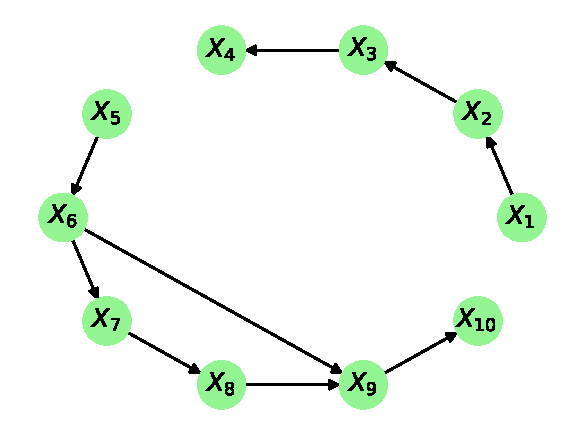
\includegraphics[width=.95\linewidth]{figures/Gaussian Chain Theoretical/Chain graph from triangular G obs - MI - cutoff 2_1e-2.pdf}
        \caption{}
        % \label{fig:Gaussian 3x3 large s}
    \end{subfigure}
    \\[\baselineskip]
    \begin{subfigure}[t]{0.49\textwidth}
        \centering
        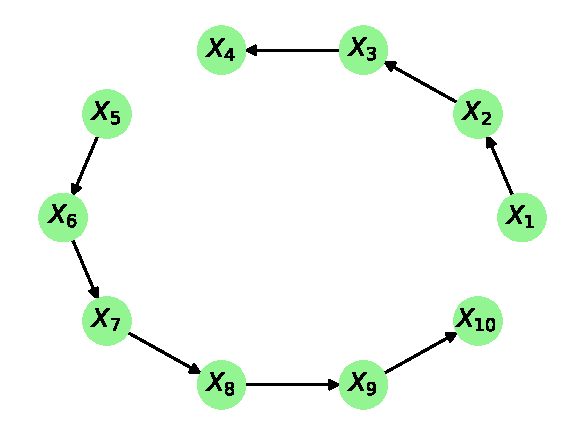
\includegraphics[width=.95\linewidth]{figures/Gaussian Chain Theoretical/Chain graph from triangular G obs - MI - cutoff 4_51e-2.pdf}
        \caption{}
        % \label{fig:Gaussian 3x3 large s}
    \end{subfigure}
    \caption{Triangular, mutual information, cutoff $2\cdot 10^{-10}$, $2.1 \cdot 10^{-2}$ and $4.51 \cdot 10^{-2}$.}
    \label{fig:Gaussian chain symmetric G_obs using mutual information different cutoff}
\end{figure}


\newpage
\section{Gaussian network deconvolution}
\begin{figure}[H]
    \centering
    \begin{subfigure}[t]{0.49\textwidth}
        \centering
        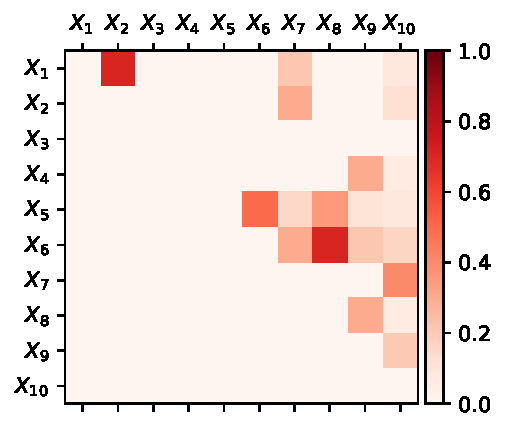
\includegraphics[width=.95\linewidth]{figures/Gaussian Network Theoretical/triangular G obs - cor.pdf}
        \caption{$G_{obs}$}
        % \label{fig:Gaussian 3x3 large s}
    \end{subfigure}
    \hfill
    \begin{subfigure}[t]{0.49\textwidth}
        \centering
        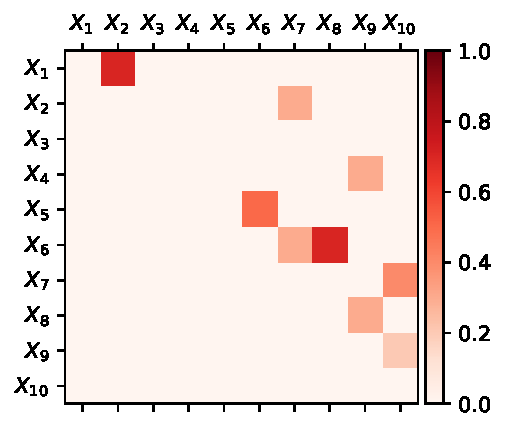
\includegraphics[width=.95\linewidth]{figures/Gaussian Network Theoretical/G dir from triangular G obs - cor.pdf}
        \caption{$G_{dir}$}
        % \label{fig:Gaussian 3x3 large s}
    \end{subfigure}
    \\[\baselineskip]
    \begin{subfigure}[t]{0.49\textwidth}
        \centering
        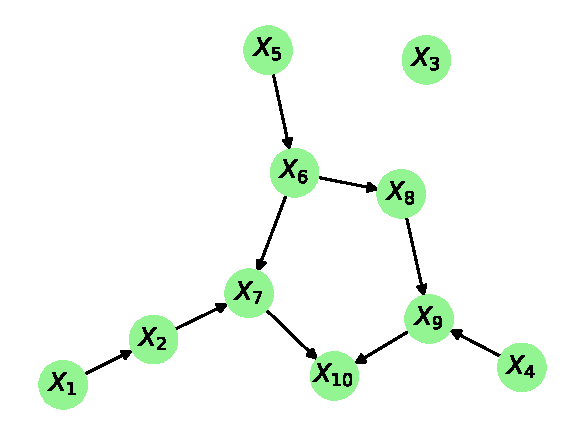
\includegraphics[width=.9\linewidth]{figures/Gaussian Network Theoretical/Graph from triangular G obs - cor.pdf}
        \caption{$G_{dir}$ as a graph}
        % \label{fig:Gaussian 3x3 large s}
    \end{subfigure}
    \caption{For the linear network defined in \autoref{eq:example Gaussian network}, using a triangular $G_{obs}$ (a) with the true topological structure we are able to perfectly rediscover the causal structure as seen in (b) and (c).}
    \label{fig:Gaussian network triangular G_obs using correlation}
\end{figure}

\end{document}                                 %Appendix A
%-----------
% Backmatter
%-----------
\backmatter
\chaptermark{Bibliography}
\renewcommand{\sectionmark}[1]{\markright{#1}}
\sectionmark{Bibliography}
\addcontentsline{toc}{chapter}{Bibliography}        %Force addition of Bibliography to TOC
\bibliographystyle{alpha}                           %Use alpha codes for references
\bibliography{References}                           %Bibliography file called
\end{document}
% % % EOF % % %